% Chapter Template

\chapter{Overview of Haptic Feedback} % Main chapter title

\label{Chapter3}

Computer Haptic Feedback or Haptics, in short, is the research field that deals with the need to be able to \textbf{digitalize the human sense of touch and reproduce it}. Despite the research done in this field since the mid-20\textsuperscript{th} century, the technology is still in its \textbf{infancy}. The main reason for this is the \textbf{complexity of the human sense of touch} which we still don't understand fully.
This, in turn, doesn't allow us to even approximately match the capabilities of the human sense of touch; but we can still use this infant technology to reproduce \textbf{simple sensations}.
Simple sensation reproduction can still be used in many fields, from the \textbf{entertainment} industry to the \textbf{medical field}, from the \textbf{military} to the \textbf{automotive industry} to \textbf{convey information that we do not normally acquire via touch}, such as notifications and warnings related to particular events, guidance instructions, and even crude reproduction of textures.
In this chapter, we will give an overview of the human sense of touch and the state of art technologies used to reproduce it.

%----------------------------------------------------------------------------------------
%	SECTION 1
%----------------------------------------------------------------------------------------
\section{Physics of Haptic Feedback}
\label{Introduction_Haptics}


% -- Subsection 1
\subsection{Biology of Haptic Sensing}
The human tactile sensing system can measure specific properties of materials, such as
temperature, texture, shape, force, fine-form features, mass distribution, friction, hardness
and viscoelasticity, through physical contact between the human skin and the object.
Even the changing state of the interaction, such as gravitational and inertial effects, can
be perceived through the sense of touch. 
As the sensing system works through the skin, it doesn't rely on a localized sensory organ but behaves as a distributed system, also different parts of the body have different thresholds of sensitivity.
For these reasons, it's difficult to treat a tactile signal as a well-defined quantity like visual and
audio signals and its complex nature makes it difficult to replicate its functioning in
science or engineering tasks.

The sense of touch is based on the somatosensory system, which is a complex system of nerve endings and touch receptors in the skin. The somatosensory system is composed of four main types of receptors:
\begin{itemize}
    \item \textbf{Mechanoreceptors} - These are the most common type of tactile receptors in the skin. They are responsible for sensing pressure, vibration, stretching, and brushing.
    \item \textbf{Thermoreceptors} - These receptors are responsible for sensing temperature changes in the skin. There are two main types of thermoreceptors: warm receptors and cold receptors.
    \item \textbf{Nociceptors} - These receptors are responsible for sensing pain and tissue damage. They are activated by noxious stimuli, such as extreme temperatures, pressure, or chemicals.
    \item \textbf{Proprioceptors} - These receptors are responsible for sensing the position and movement of the body. They are located in the muscles, tendons, and joints, and provide feedback to the brain about the relative position between different parts of the body.
\end{itemize}

The most important receptors for haptic feedback are the mechanoreceptors, they react to mechanical stimuli by producing signals in the form of streams of voltage pulses at high frequencies, the stronger the stimuli higher the frequency of the pulses. When the cell adapts to the stimulus, the pulse frequency subsides to its normal rate.
Considering the goal of this research we can focus on the mechanoreceptors that are responsible for sensing pressure and vibration, these are the Pacinian corpuscles and the Meissner corpuscles.
The first ones are more sensible to high-frequency vibrations (200-550Hz), while the second ones are more for low-frequency vibrations (20-40Hz). \cite{Alg_Wearable_Tech_Nicole}

% -- Subsection 2
\subsection{Haptic sensitivity}
\label{Haptic sensitivity}

As the mechanoreceptors are \textbf{enveloped in various skin layers}, their sensitivity to vibrations will not be infinite. The \textbf{strength of the sensation} will depend on the \textbf{frequency} and \textbf{amplitude of the vibration}. 

The \textbf{amplitude} of the vibration can be considered in \textbf{terms of the acceleration of the membrane-magnet system}.

Previous works \cite{Vibrotactile_Sensitivity} found that, for a pulp contact area ranging from 53 to 176.7 mm\textsuperscript{2}, the threshold of detection of vibrations was between 0.1778 and 0.5623 m/s\textsuperscript{2} (in the work specified as 105-115 dB (re 1e-6m/s\textsuperscript{2})) for sinusoidal stimuli ranging from 100 to 250 Hz. 
For frequencies close to \textbf{125Hz} the threshold should also \textbf{lower} as the finger pulp reaches its \textbf{resonance frequency} \cite{Skin_freqs_penetration}.

The study also highlights that the sensitivity depends on the \textbf{constant pressure force applied on the skin} in conjunction with the vibration.
They found that under active pressing force, the sensitivity threshold decreases to 0.027-0.143 m/s\textsuperscript{2} (in the work specified as 68.5-83.1 dB (re 1e-6m/s\textsuperscript{2})) for a constant applied force of 1.6N.

\begin{samepage}
    For higher pressure forces the sensitivity threshold decreases even further, as we can observe in Fig. \ref{fig: Vibrotactile_Sensitivity}.
    \begin{figure}[H]
        \centering
        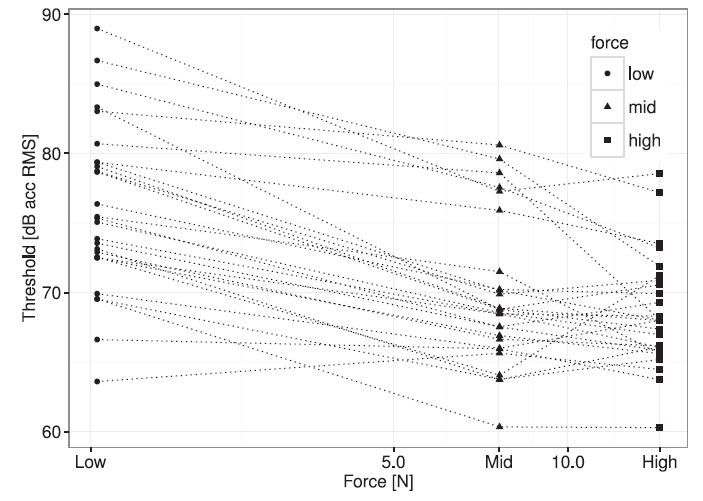
\includegraphics[width=0.5\linewidth]{Chapters/Chapter3/Haptics_Physics/Figures/vibr_thr_vs_pressure_force.png}
        \caption{Sensitivity as a function of the applied pressure \cite{Skin_freqs_penetration}.}
        \label{fig: Vibrotactile_Sensitivity}
    \end{figure}
\end{samepage}



%----------------------------------------------------------------------------------------
%	SECTION 2
%----------------------------------------------------------------------------------------
\section{State of the Art in vibrotactile haptic feedback}
For now, state of the art in haptic feedback is still in its infancy.
The main reason for this is the complexity of the human sense of touch which we still don't understand fully.
The \textbf{best technology} we have for now to reproduce haptic feedback through \textbf{vibrotactile} means is the \textbf{piezoelectric actuator}.

% --- SUBSECTION 1
\subsection{Piezoelectric actuators}
Piezoelectric actuators are a very interesting technology based on the \textbf{piezoelectric effect}.
Materials exhibiting this effect, such as certain ceramics and crystals, possess the ability to \textbf{convert electrical energy into mechanical motion}, and vice versa.

The operating principle of piezoelectric actuators relies on the application of an electric field across the piezoelectric material. This electric field induces a \textbf{deformation within the material}, causing it to expand or contract depending on the polarity of the applied voltage. This minute deformation translates into \textbf{highly precise mechanical displacement}, enabling piezoelectric actuators to achieve nanometer-scale resolutions with \textbf{remarkable speed and accuracy}.

One of the defining characteristics of piezoelectric actuators is their \textbf{rapid response time}. Unlike traditional electromagnetic actuators, which may suffer from inertia and mechanical backlash, piezoelectric actuators can swiftly change their state in response to electrical signals.

\subsubsection{Frequency response}
Piezoelectric actuators are perfect for haptic applications as they can provide a \textbf{wide range of frequencies}.
Piezo specifically engineered for haptic feedback can provide a frequency range from 1 Hz to 1 kHz. \\

All piezoelectric actuators have a natural frequency at which they resonate. This \textbf{frequency} is determined by the \textbf{mechanical properties} of the actuator, such as its mass and stiffness, as well as the electrical properties of the piezoelectric material.

\begin{samepage}
    The important thing to note is that this \textbf{frequency also depends on the load} that the actuator is driving:
    \nopagebreak

    \begin{equation}
        f_{res} = \frac{1}{2\pi} \sqrt{\frac{k}{m_{eff}+m_{load}}}
    \end{equation}
    \nopagebreak

    Where:
    \nopagebreak

    \begin{itemize}
        \item \( f_{res} \) = Resonant frequency [Hz]
        \item \( k \) = Stiffness of the piezo actuator [N/m]
        \item \( m_{eff} \) = Effective mass of the actuator [kg]
        \item \( m_{load} \) = Mass of the load [kg]
    \end{itemize}
\end{samepage}


As the frequency of the actuator approaches its resonant frequency, the \textbf{amplitude} of the actuator's motion \textbf{increases significantly}. This phenomenon must be taken into account when designing a control system for the piezo actuator, as at maximum voltage the actuator could be \textbf{damaged} if in resonance.

\subsubsection{Force performances}
Taking as an example a piezo actuator built specifically for haptic feedback, the PowerHap series from TDK \cite{Piezo_Haptic_Actuator}, we can see that the actuator can provide a force up to \textbf{20N} in a frequency range from 1 Hz to 500Hz.

\subsubsection{Power consumption}
Considering still as an example the PowerHap series from TDK, we can read from the datasheet that the actuator can be run with a peak voltage of 120V and an average current of 0.432A (calculated using \cite{Power_piezo_calculator} in the case of a square wave signal of 500Hz). This means that the actuator can \textbf{consume} up to \textbf{25.9W} of power at its peak frequency.
In the same condition, it will also \textbf{dissipate} about \textbf{2.59W} of power as heat.

% % --- SUBSECTION 2
\subsection{Texture rendering} % TODO: Decide if this section is needed
\begin{itemize}
    \item frequency requirements
    \item force requirements
    \item response time
\end{itemize}



%----------------------------------------------------------------------------------------
%	SECTION 4
%----------------------------------------------------------------------------------------
%\section{Performance comparison between Piezo and Coil's actuators}

% % -- Subsection 2.1
% \subsection{Force and displacement}

% % -- Subsubsection 2.2
% \subsection{Frequency response} %TODO: decide if to include this section